\section{Vererbung}

{\setbeamertemplate{footline}{\parbox{\linewidth}{\vspace*{-8pt}Quelle: \url{https://de.wikipedia.org/wiki/Vererbung_(Programmierung)}}}
\begin{frame}
	\frametitle{Vererbung}
	\begin{itemize}
		\item Meist in Kombination mit Polymorphie
		\item Eigenschaften und Methoden der Basisklasse A werden in abgeleitete Klasse B übernommen
		\item Doppelter Code und Schreibarbeit werden vermieden
		\item UML: Pfeil von abgeleiteter Klasse zu Basisklasse
	\end{itemize}
	\begin{figure}[h]
		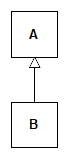
\includegraphics[scale=0.75]{vererbung/uml.png}
	\end{figure}
\end{frame}
}

{\setbeamertemplate{footline}{\parbox{\linewidth}{\vspace*{-8pt}Quelle: \url{https://de.wikipedia.org/wiki/Vererbung_(Programmierung)\#Datenkapselung_im_Rahmen_der_Vererbung}}}
\begin{frame}
	\frametitle{Datenkapselung im Rahmen der Vererbung}
	\begin{figure}[h]
		\begin{table}[H]
	\begin{tabularx}{\textwidth}{$l|^X|^X|^X}
		\multicolumn{4}{l}{\bfseries Sichtbarkeit in ...} \\
		\hline
		\bfseries Basisklasse    & \multicolumn{3}{l}{\bfseries abgeleiteter Klasse (erbt ... von Basisklasse)} \\
		\rowstyle{\bfseries}     & öffentlich    & geschützt                   & privat                      \\
		                         & (``ist-ein'') & (``ist-implementiert-mit'') & (``ist-implementiert-mit'') \\
		\hline
		öffentlich $\rightarrow$ & öffentlich    & geschützt                   & privat                      \\
		geschützt  $\rightarrow$ & geschützt     & geschützt                   & privat                      \\
		privat     $\rightarrow$ & nicht vererbt & nicht vererbt               & nicht vererbt               \\
	\end{tabularx}
\end{table}

	\end{figure}
	\begin{itemize}
		\item Layering: ``hat-ein''-/''ist-implementiert-mit''-Beziehung
	\end{itemize}
\end{frame}
}

{\setbeamertemplate{footline}{\parbox{\linewidth}{\vspace*{-8pt}Vollständiger Code: \url{https://godbolt.org/z/neqhe7GsG}}}
\begin{frame}
	\frametitle{Beispiel:}
	{\tiny\UseRawInputEncoding{\lstinputlisting[language={C++}]{vererbung/beispiele/point/src/point2d.hpp}}\inputencoding{utf8}}
	\pause
	{\bfseries Lösung ohne Vererbung:}
	{\tiny\UseRawInputEncoding{\lstinputlisting[language={C++}]{vererbung/beispiele/point/src/point3d.no.hpp}}\inputencoding{utf8}}
	\pause
	{\bfseries Lösung mit öffentlicher Vererbung:}
	{\tiny\UseRawInputEncoding{\lstinputlisting[language={C++}]{vererbung/beispiele/point/src/point3d.public.hpp}}\inputencoding{utf8}}
	\pause
	{\tiny\UseRawInputEncoding{\lstinputlisting[language={C++}]{vererbung/beispiele/point/src/point.use.cpp}}\inputencoding{utf8}}
	\pause
	{\bfseries Lösung mit privater Vererbung:}
	{\tiny\UseRawInputEncoding{\lstinputlisting[language={C++}]{vererbung/beispiele/point/src/point3d.private.hpp}}\inputencoding{utf8}}
\end{frame}
}


{\setbeamertemplate{footline}{\parbox{\linewidth}{\vspace*{-8pt}Quelle: \url{https://de.wikipedia.org/wiki/Vererbung_(Programmierung)\#Schnittstellenvererbung}}}
\begin{frame}
	\frametitle{Schnittstellenvererbung}
	\begin{itemize}
		\item Nur Methodensignatur, aber keine Standardimplementierung, wird vererbt
		\item Java: Interface
		\item C++: abstrakte Klasse, die nur rein virtuelle Methoden enthält
	\end{itemize}
\end{frame}
}

{\setbeamertemplate{footline}{\parbox{\linewidth}{\vspace*{-8pt}Quelle: \url{https://de.wikipedia.org/wiki/Vererbung_(Programmierung)\#Implementierungsvererbung}}}
\begin{frame}
	\frametitle{Implementierungsvererbung}
	\begin{itemize}
		\item Methodensignatur und Standardimplementierung werden vererbt
		\item Standardimplementierung kann aber von abgeleiteter Klasse überschrieben werden
	\end{itemize}
\end{frame}
}


{\setbeamertemplate{footline}{\parbox{\linewidth}{\vspace*{-8pt}Quelle: \url{https://en.wikipedia.org/wiki/Multiple_inheritance}}}
\begin{frame}
	\frametitle{Mehrfachvererbung}
	\begin{itemize}
		\item Eine abgeleitet Klasse erbt von mehreren Basisklassen
		\item Mehrfachinterfacevererbung problemlos möglich
		\item Mehrfachimplementierungsvererbung führt oft zu fehleranfälligem und unübersichtlichem Code
	\end{itemize}
	\begin{figure}[H]
		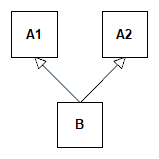
\includegraphics[scale=0.75]{vererbung/mehrfach/mehrfach.png}
	\end{figure}
\end{frame}
}

{\setbeamertemplate{footline}{\parbox{\linewidth}{\vspace*{-8pt}Quelle: \url{https://de.wikipedia.org/wiki/Diamond-Problem}}}
\begin{frame}
	\frametitle{Diamond-Problem}
	\begin{itemize}
		\item Eine abgeleitete Klasse erbt über mehr als einen Pfad von derselben Basisklasse
		\item Eigenschaften und Methoden werden mehrfach vererbt
	\end{itemize}
	\begin{figure}[H]
		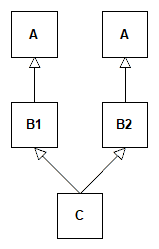
\includegraphics[scale=0.75]{vererbung/mehrfach/diamond/nicht_virtuell.png}
	\end{figure}
\end{frame}
}

{\setbeamertemplate{footline}{\parbox{\linewidth}{\vspace*{-8pt}Quelle: \url{https://de.wikipedia.org/wiki/Diamond-Problem\#Modellierung_in_C++}}}
\begin{frame}
	\frametitle{Virtuelle Vererbung (C++)}
	\begin{itemize}
		\item B1 und B2 erben von A virtuell
		\item abgeleitete Klassen teilen sich eine gemeinsame Instanz
	\end{itemize}
	\begin{figure}[H]
		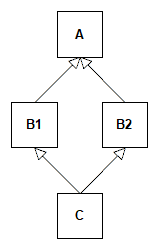
\includegraphics[scale=0.75]{vererbung/mehrfach/diamond/virtuell.png}
	\end{figure}
\end{frame}
}

\begin{frame}
	\frametitle{Beispiel -- Schüler/Lehrer}
	\begin{itemize}
		\item Schüler und Lehrer erben von Person
		\item Es gibt auch Schüler, die anderen Schülern Nachhilfe geben
	\end{itemize}
	\begin{figure}[H]
		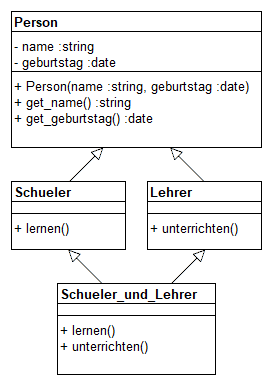
\includegraphics[scale=0.5]{vererbung/mehrfach/diamond/beispiele/schueler_lehrer/schueler_lehrer.png}
	\end{figure}
\end{frame}


{\setbeamertemplate{footline}{\parbox{\linewidth}{\vspace*{-8pt}Vollständiges Beispiel: \url{https://godbolt.org/z/5Kqe1cG93}}}
\begin{frame}
	\frametitle{Abstrakte Klassen}
	\begin{itemize}
		\item Von abstrakten Klassen können keine Objekte erzeugt werden
		\item Es wird geerbt und von der abgeleiteten Klasse ein Objekt erzeugt
	\end{itemize}
	
	{\scriptsize\bfseries Java:}
		{\tiny\UseRawInputEncoding{\lstinputlisting[language={Java}]{vererbung/abstrakt/abstrakt.java}}\inputencoding{utf8}}
	
	{\scriptsize\bfseries C++:}
		{\tiny\UseRawInputEncoding{\lstinputlisting[language={Java}]{vererbung/abstrakt/abstrakt.hpp}}\inputencoding{utf8}}
		
		\pause{\tiny\UseRawInputEncoding{\lstinputlisting[language={Java}]{vererbung/abstrakt/abstrakt.use.cpp}}\inputencoding{utf8}}
		
		\pause{\tiny\UseRawInputEncoding{\lstinputlisting[language={Java}]{vererbung/abstrakt/abgeleitete_klasse.hpp}}\inputencoding{utf8}}
		{\tiny\UseRawInputEncoding{\lstinputlisting[language={Java}]{vererbung/abstrakt/abgeleitete_klasse.use.cpp}}\inputencoding{utf8}}
\end{frame}
}

{\setbeamertemplate{footline}{\parbox{\linewidth}{\vspace*{-8pt}Vollständiges Beispiel: \url{https://godbolt.org/z/fnbKh1Pr9}}}
\begin{frame}
	\frametitle{Endgültige Klassen}
	\begin{itemize}
		\item Kann keine Basisklasse sein
	\end{itemize}
	
	{\tiny\UseRawInputEncoding{\lstinputlisting[language={Java}]{vererbung/endgueltig/endgueltig.hpp}}\inputencoding{utf8}}
	{\tiny\UseRawInputEncoding{\lstinputlisting[language={Java}]{vererbung/endgueltig/abgeleitete_klasse.hpp}}\inputencoding{utf8}}
\end{frame}
}
